\chapter{Cloud}
Cloud came out as a business model, not as a technlogy.
It was needed to handle peak of requests and to allow scalability, without oversizing Infrastructures.
\note{e.g. Amazon needs to handle way more requests on Christmas than on a normal day.}
So, Cloud was a mean to reduce the cost of the ICT infrastructure.

\note{When you program for the cloud, the consumer don't know where the process will be executed or where the data will be stored.}

\textbf{Resource pooling} is the key concept of Cloud. It means that the services are provided to users using a multi-tenant model, with physical and virtual resources being dynamically allocated and deallocated according to the demand.\\
Cloud was needed also to provide rapid \textbf{elasticity}, meaning that capabilities may be elastically provisioned and released, in some cases automatically, to scale rapidly outward and inward commensurate with demand. 
To the customer it means that the capabilities available for provisioning often appear to be unlimited and can be appropriated in any quantity at any time.

\textbf{Resource measurement} is another fundamental pillar of Cloud: since the Cloud model revolves around pricing and resource consumption it's imperative to monitor and measure the usage of resources.

Benefits of Cloud:
\begin{itemize}
   \item \textbf{Business agility}
   \begin{itemize}
      \item Quick resource provisioning
      \item Facilitates innovation
      \item Reduces time to market
   \end{itemize}
   \item \textbf{Reduces IT costs}
   \begin{itemize}
      \item Reduces up-front capital expenditure (CAPEX)
      \item Improves resource utilization
      \item Reduces operational expenditure (OPEX)
   \end{itemize}
   \item \textbf{High availability}
   \begin{itemize}
      \item Ensure resource availability based on customer's requirements
      \note{In RAI, prof. Cisternino experienced people complaining because their servers' CPUs were running at 98\% of their capability, and they wanted to exploit also the remaining 2\%, because ``they paid for it''.}
      \item Enables fault tolerance
      \note{Recall active-active, active-passive, etc. configurations.}
   \end{itemize}
   \item \textbf{Business continuity}
   \item \textbf{Flexible Scaling}
   \item \textbf{Flexibility of Access}
   \item \textbf{Application Dev and Testing}
   \item \textbf{Simplified infrastructure management}
   \item \textbf{Increased collaboration}
   \item \textbf{Masked complexity}
\end{itemize}
Cloud has the magic power of decoupling the software from the hardware.

Disadvantages of Cloud:
\begin{itemize}
   \item Vendor lock-in
   \item Privacy
   \item Your software depends on someone else
   \item Legislation is complicated
   \note{In EU public administration data, must be stored in the EU.}
   \item \dots TODO
\end{itemize}

\section{Cloud Service Models}
\begin{itemize}
   \item \textbf{IaaS} (Infrastructure as a Service)
   \begin{itemize}
      \item Provides virtualized computing resources over the Internet
      \item Examples: Amazon EC2, Google Compute Engine, Microsoft Azure
   \end{itemize}
   \item \textbf{PaaS} (Platform as a Service)
   \begin{itemize}
      \item Provides a platform allowing customers to develop, run, and manage applications without the complexity of building and maintaining the infrastructure
      \item Examples: Google App Engine, Microsoft Azure, Heroku
   \end{itemize}
   \item \textbf{SaaS} (Software as a Service)
   \begin{itemize}
      \item Provides software applications over the Internet
      \item Examples: Google Apps, Microsoft Office 365, Salesforce
   \end{itemize}
\end{itemize}

\section{Cloud Deployment Models}
\begin{itemize}
   \item \textbf{Public Cloud}
   \begin{itemize}
      \item Owned and operated by third-party cloud service providers
      \item Deliver computing resources over the Internet
      \item Examples: Amazon Web Services (AWS), Microsoft Azure, Google Cloud Platform
   \end{itemize}
   \note{It does \textbf{not} mean that the data is public. It means that the cloud services are accessible to the public.}
   \item \textbf{Private Cloud}
   \begin{itemize}
      \item Operated solely for a single organization
      \item Managed by the organization or a third party
      \item \textit{On-premise} or \textit{off-premise}
   \end{itemize}
   \note{It does \textbf{not} mean that the data is private. It means that the cloud services are accessible only to the organization e.g. \textit{UniPi}.}
   \item \textbf{Hybrid Cloud}
   \begin{itemize}
      \item Composition of two or more clouds (private, community, or public) that remain unique entities but are bound together, and resources may be moved from one cloud to another (with some performance cost obviously) 
      \item By standardized or proprietary technology that enables data and application portability
   \end{itemize}
   \item \textbf{Community Cloud}
   \begin{itemize}
      \item Shared infrastructure for specific community
      \item Managed by organizations or third party
      \item On-premises or off-premises
   \end{itemize}
\end{itemize}

\newpage
\section{Cloud as a Layered architecture - Cisternino's POV}
\begin{figure}[htbp]
   \centering
   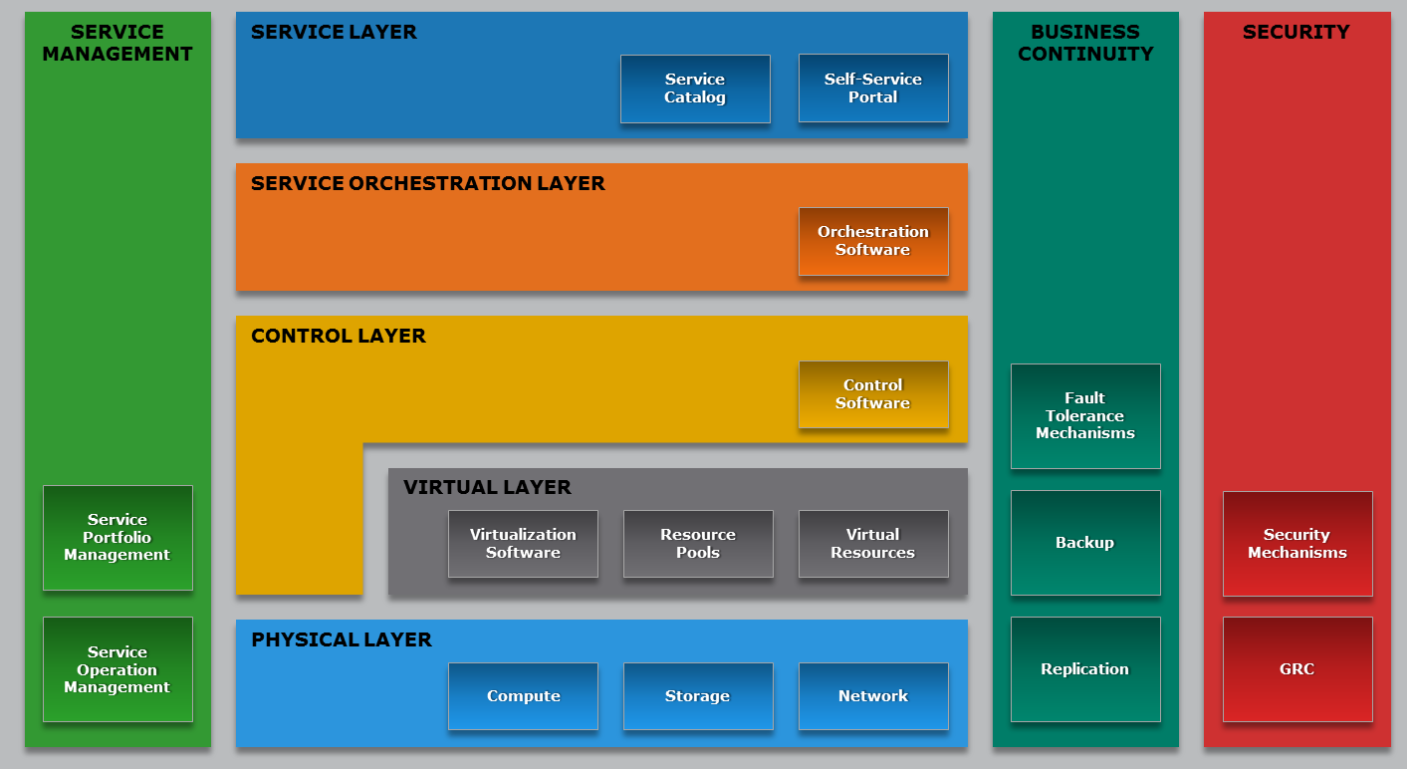
\includegraphics{images/cloud_layers.png}
   \caption{Cloud infrastructure as a layered architecture}
   \label{fig:cloud_layers}
\end{figure}
In the last lectures of the Course, prof. Cisternino introduced the Cloud as a layered architecture, where each layer is responsible for a specific task, but went deeper only into the following topics:
\begin{itemize}
   \item Software for control layer resource management
   \item Workflows: formalism to describe orchestration processes
   \item RPO and RTO key metrics
   \item The first two pages of Security
   \item Zero Trust Architecture
   \item Service Level Agreement
   \item Incident and Problem management
\end{itemize}
% // TODO ref to sections
\newpage

\section{Physical Layer}
Comprises \textbf{compute}, \textbf{storage} and \textbf{network} resources and executes both provider and consumer software. Compute systems are offered in the form of virtual machines.\\
Storage and access methods (e.g. file-based, unified, \dots) have been exhaustively discussed in previous chapters.\\
For what concerns the network communications, they may be:\ns
\begin{itemize}
   \item \textbf{Compute-to-Compute} (East-West?\footnote{Perhaps not necessarily}) : typically uses IP-based protocols
   \item \textbf{Compute-to-Storage} : typically a SAN exploiting depending on the fabric and architecture SCSI, iSCSI, FC, FCoE, NFS, SMB, etc.\\
   \begin{itemize}
      \item FC SAN: Fibre Channel provinding up to 16Gbps bandwidth, and block-level access to storage
      \item IP SAN: SAN using IP protocol and iSCSI or FCIP on top of it. Both encapsulate, respectively, SCSI and FC frames into IP packets
      \item FCoE SAN: Fibre Channel over Ethernet
   \end{itemize}
   \item \textbf{inner-cloud}: A different cloud interconnected to another one by WAN.
\end{itemize}

\section{Virtual Layer}
Abstract physical resources, including storage and network, and makes them appear as virtual resources.
\framedt{Virtualization}{
   Through \textbf{virtualization} a multi tenant environment is achieved, by running multiple ---customer--- organizations VMs on the same server;
   note however that this concept is not limited to VMs as a computing resource, but applies to storage and network as well.
   Virtual LANs, SANs and switches may be created.

   Virtualization is composed by 3 entities:\ns
   \begin{itemize}
      \item Virtualization Software
      \item Resource pool
      \item Virtual resources
   \end{itemize}
}
\nl

Lastly, remember that Hypervisors, used to manage VMs and virtual resources, may be of two types:
\begin{itemize}
   \item \textbf{bare-metal}: directly installed on the hardware. Performes better than hosted hypervisors, and typically are designed for enterprise datacenters.
   \item \textbf{hosted}: installed on top of an OS. Unlike bare-metal hypervisors, they do not have direct access to the hardware.
\end{itemize}

\subsection{VMs network components}
\begin{enumerate}
   \item \texttt{vSwitch}: OSI Layer 2 switch that forwards traffic between VMs. May be internal or external, depending whether it connects solely VMs or if it is also attached to a physical NIC.
   \note{A physical NIC already connected to a vSwitch cannot be attached to any other vSwitch.}
   \item \texttt{vNIC}: A vNIC connects a VM to a virtual switch, acting similarly to a physical NIC. Each vNCI has a unique MAC and IP address, and uses ethernet just as a physical NIC would.
   \item \texttt{Uplink NIC}: an uplink NIC is a physical NIC connected to the uplink port of a vSwitch and functions an \textit{Inter-switch link}.
   It is called uplink because it only provides a physical interface to connect a compute system to the network and is not addressable from the network, they are neither assigned an IP address nor are their built-in MAC addresses available to any compute system in the network. 
   They simply forward the VM traffic between the VM network and the external physical network without modification.
\end{enumerate}

\subsection{Virtual Networks}
\begin{enumerate}
   \item VLAN
   \item PVLAN (Private VLAN)
   \item Stretched VLAN 
   \item VXLAN (Virtual Extensible LAN)
   \item VSAN
\end{enumerate}
There exists a mapping between VSAN and VLAN to determine which VLAN carries a VSAN traffic.


\section{Control Layer}
The control layer is responsible for managing the resources and the allocation of the resources to the virtual machines.

\begin{definition}[Control Layer]
   ``The control layer is important because it's the way pool the resources set and see all the resources in a coherent way so it's a sort of a software layer that hides the differences and gives you primitives (such as ``I need a VM, I don't care where, but I need one'').''
\end{definition}


Note that you cannot allocate more virtual cores than the physical ones ---same applies to memory---, but you can allocate smaller pieces so you can create a resource pooling of resources that can be taken partially (assuming that they can run on a single node), but making you perceive it as a pool of resources.

\textit{Service} and \textit{Orchestration} layers above the control layer have no clue where workloads are running, they just send requests to the control one, it is completely up to such layer to manage where and how. 
\nl

The steps towards provisioning a resource are three
\begin{enumerate}
   \item \textbf{Resource Discovery}
   \item \textbf{Resource Pooling}
   \item \textbf{Resource Provisioning}
\end{enumerate}

A key component in the control layer is a Unified Manager software, which handles, by means of APIs, the tools associated to
\begin{itemize}
   \item Compute System management
   \item Fabric management
   \item Storage System management
\end{itemize}

\subsection{Resource Discovery}
The control layer enables \textbf{unified manager} to learn about resources that are available for service deployment
Provides visibility to each resource
Enables to manage cloud infrastructure resources centrally


\subsection{Resource Pooling and Provisioning}
A unified manager at control layer allows to categorize in \textbf{grading pools} resources and identity pools based on predefined criteria.
This helps creating variety of services decoupled from the actual hardware where they will run, but still providing choices to consumers on the type ---and amount--- of hardware they get (e.g. ``0.5TB Flash, 4TB SATA, 1TB FC'').
Multiple grade levels (e.g. ``Gold'', ``Silver'', ``Bronze'') may be defined for each type of pool, where costs/prices of resource pools differ depending on grade level.
\nl

\framedt{Resource provisioning starts when a user requests a service.}
{
   When I create a VM, i can choose the template (e.g. ``Windows 2016'', ``Ubuntu 18.04''), hardware, extensions, and lastly I will be asked to select a Host.
   At that point the system polls the control layer to see which hosts are available and which are not, and then rank them.
   Then I'll be asked for the chosen host the estimated workload on CPU (percentage), memory and disk.
   Set the host, the control software provides information regarding networking.
}

Lastly, it is important to recall that \textbf{Resource monitoring} is fundamental to keep track of the resources used and to prevent over-provisioning.

\newpage
\subsection{Control Software demo}

\begin{paracol}{2}
   \colfill
   Prof. Cisternino demonstrated a Control Software he uses for the UniPi Cloud, where he can see the resources available and the resources allocated to the VMs.
   
   In the ``VM and Services'' view, the software allows to see the different Clouds associated to Polo 1, Polo 2, etc. and the resources allocated to each of them.\\
   There is also another inner view to check VM networks and the actual hosts where the VMs are running.
   
   He may even open a Powershell terminal on a VM.

   \ul{This software allows him to manage about 1400 VMs.}
   \colfill
   \switchcolumn
   \begin{figure}[htbp]
      \centering
      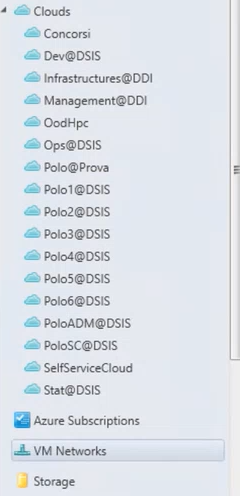
\includegraphics[width=0.45\columnwidth]{images/Control_VMandServices.png}
      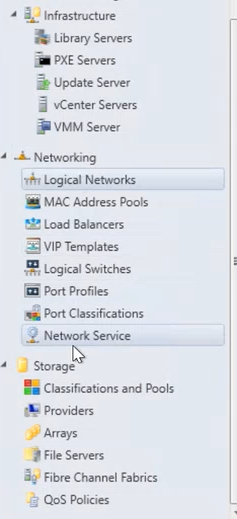
\includegraphics[width=0.45\columnwidth]{images/Control_FabricView.png}
      \caption{VM and Services view}
   \end{figure}
   \end{paracol}

   
\section{Service Layer/Service Orchestration Layer}

\begin{definition}[Cloud Service]
   \label{def:cloudservice}
   IT resources that are packaged by the service providers and are offered to the consumers
\end{definition}
This means that deploying a service, does not mean simply deploying a VM, but a bunch of them, and also configuring it, installing software, etc. 

\textbf{Service Layer} enables defining services in a service catalog, and provides a self-service portal for users to request services (enables on-demand and self-provisioning).
\note{Essentially, the catalog is the DB while the cloud portal is the web interface for it.}

\subsection{Service Orchestration Layer}
\textbf{Service Orchestration layer} implements the process of integrating services to support the automation of business processes:
\ul{actuates the policies and the requests automatically from the user}.

\begin{definition}[Tenant] A tenant is a user of the cloud, and the cloud provider must ensure that the tenant is isolated from the others. This is done by means of \textbf{multi-tenancy}.
\end{definition}
\note{UniPi\st{.it} is a tenant for Microsoft Azure.}
\subsubsection*{Workflows}
\begin{figure}[htbp]
   \centering
   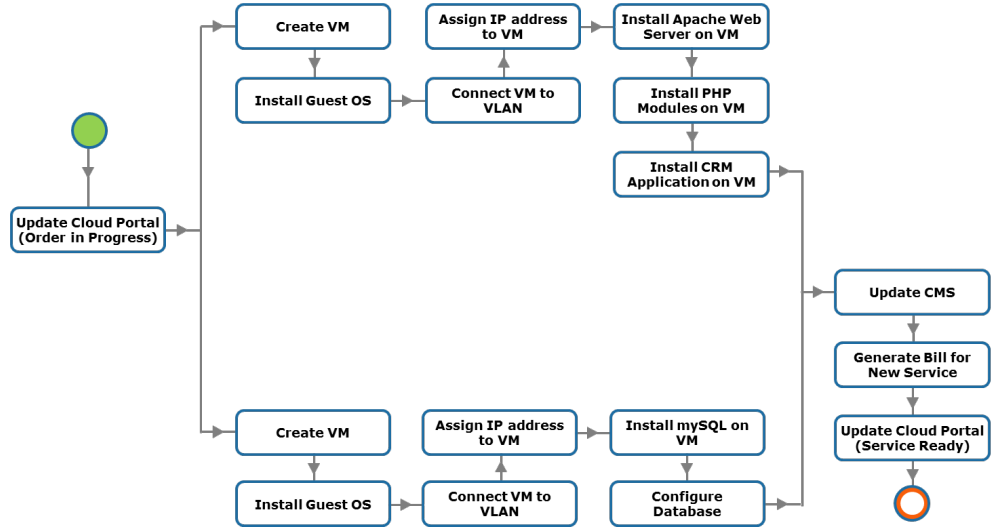
\includegraphics[width=0.45\columnwidth]{images/serviceorchestration1.png}
   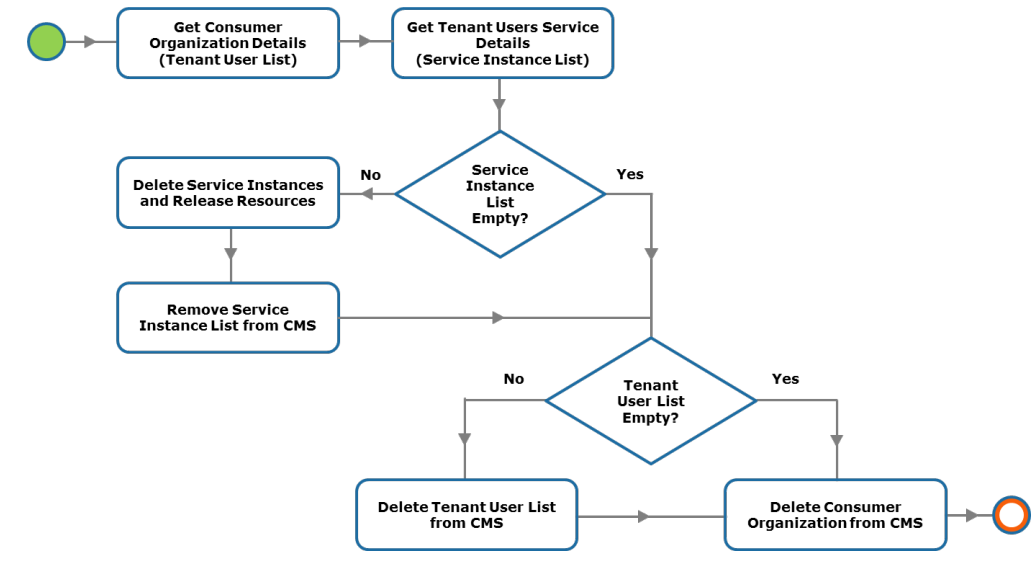
\includegraphics[width=0.45\columnwidth]{images/serviceorchestration2.png}
   \caption{Service orchestration layer use cases. On the left, provisioning a CRM application, while on the right a tenant removal}
   \label{fig:serviceorchestration}
\end{figure}

Although some manual steps (performed by cloud administrators) may be
required while processing the service provisioning and management
functions, service providers are looking to \textbf{automate these
functions as much as possible}.

Cloud service providers typically deploy a purpose-designed orchestration software (\textit{``orchestrator''}) that orchestrates the execution of various system functions.
The \textbf{orchestrator} \ul{programmatically integrates and sequences various system functions into automated workflows for executing higher-level service provisioning} and management functions provided by the cloud portal.\\
The orchestration workflows are not only meant for fulfilling requests from consumers but also for administering cloud infrastructure, such as adding resources to a resource pool, handling service-related issues, scheduling a backup for a service, billing, and reporting.

\subsection{Deeper into Services}
\begin{paracol}{2}

   We may generalize the \ul{\textbf{lifecycle} of a service} as it is depicted in Figure \ref{fig:servicelifecycle}, split in 4 main phases:
   \ns
   \begin{enumerate}
      \item \textbf{Planning}
      \begin{enumerate}
         \item Assessing service requirements
         \item Developing service enablement roadmap
         \item Establishing billing policy
      \end{enumerate}
      \item \textbf{Creation}
      \begin{enumerate}[ref=\theenumi{}.\roman*]
         \item Defining service template
         \item Creating orchestration workflow
         \item Defining service offering
         \item Creating service contract\label{enum:SLA}
      \end{enumerate}
   \end{enumerate}
   \switchcolumn
   \colfill
   \begin{enumerate}[start=3]
      \item \textbf{Operation}
      \begin{enumerate}
         \item Discovering service assets
         \item Managing service operations
      \end{enumerate}
      \item \textbf{Termination}
      \begin{enumerate}
         \item Natural termination by contract agreement
         \item Initiated termination by a provider or a consumer          
      \end{enumerate}
   \end{enumerate}
   \colfill
\end{paracol}
\begin{figure}[htbp]
   \centering
   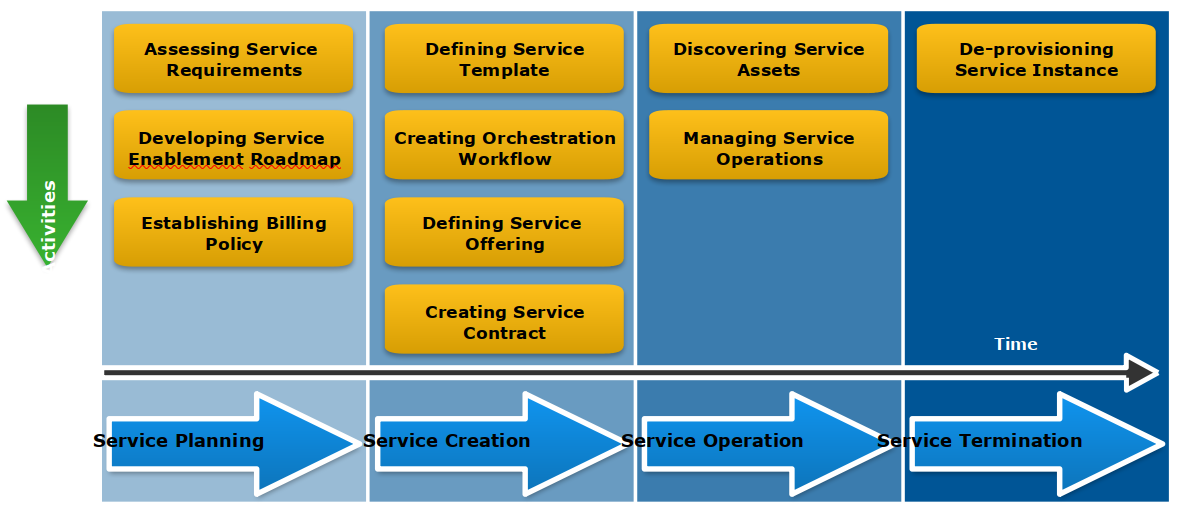
\includegraphics{images/servicelifecycle.png}
   \caption{Service Lifecycle schema}
   \label{fig:servicelifecycle}
\end{figure}

Having defined what a Service is \ref{def:cloudservice}, we can now define the \textbf{Service Layer} as the layer that provides the services to the users.

Step \ref{enum:SLA} refers ---also--- to the Service Level Agreement, which basically is the legalese version of the set of resources that we are allocating for a user.\\
Aside from the SLA, other parameters are discussed such as pricing, termination of service and possibly other configuration aspects.

\framedt{
   ``If you are smart enough you may trick the user''
}{
   Amazon tricked a user by establishing a SLA that said that the user would have a 99.999\% uptime, but they considered uptime even when the service was both not available and \textit{not} requested by the user.
}

\section{Business Continuity}
\begin{definition}[Business Continuity]
   The capability of an organization to continue delivery of products or services at acceptable predefined levels following a disruptive incident.

   \emph{\dots or \dots}
   
   BC entails preparing for, responding to, and recovering from service outage that adversely affects business operations
\end{definition}

\textbf{SPOF}s may occur at component level, or at site or data center level.\\
The key to avoid SPOFs is to have redundancy, which may be achieved by means of \textbf{replication} or \textbf{backup}s (more on this later).
\nl

\begin{definition}[Compute Clustering]
   A technique where at least two compute systems (or nodes) work together and are viewed as a single compute system to provide high availability and load balancing. 

\end{definition}
Enables service failover in the event of compute system failure to another system to minimize or avoid any service outage.\\
The implementation may be \textit{active-active} or \textit{active-passive}.

\subsection{Data Protection}
A \textbf{backup} is not simply a copy of the current data to be used in case a disk fails. In case a ransomware attack occurs, the copy will be encrypted as well, or even more trivially, if a service has a bug and it corrupts data, also the copy would contain bad data.\\
``\ul{Backup must allow to travel back in time.}''

The two critical terms are \textit{Recovery Time Objective} (\texttt{RTO}) and  \textit{Recovery Point Objective} (\texttt{RPO})\footnote{Point in time}.
They refer to the time it takes to recover from a disaster and the amount of data that can be lost respectively.

Backups are typically done incrementally, meaning that starting from a full backup, then only differences are stored.
However, saving storage in this way leads to a more complex recovery process, as all the incremental backups must be applied to the full backup to recover the data, possibly considerably increasing the RTO.\\
To overcome the issue, a full backup is done every now and then e.g. a week is common practice, and incremental daily backups are done until the next full backup.\\
This fixes the RPO to 1 day, while the RTO still may vary depending on bandwidth, storage speed, and most importantly size and amount changes throughout time; typically it is days (?) or hours.

\section{Security}
\ul{Information is an organization’s most valuable asset.}

Cloud is interesting, because, among other things, allows to distribute information in multiple places, to the cost of possibly broadening the attack surface.\\
However, cloud tenants are isolated from each other, so the attack surface is typically limited to the cloud provider's infrastructure.

For cloud customers the key point is \textbf{trust}, which is provided by means of \textbf{visibility} and \textbf{control} on the data hosted.

\framedt{Three ICT Security Pillars}{
   \begin{enumerate}
      \item \textbf{Phyisical Security}\\
      Badges, doors, locks, keys, etc\dots These are needed because with physical access to the hardware, one can do anything.
      \item \textbf{Logical Security}\\
      Accounts, passwords, firewalls, etc\dots\\
      Logical security has been historically underestimated, but it is fundamental, and it was the easier to exploit. It refers to things like access rights, restricting an account's capabilities, etc. 
      \item \textbf{Produceral Security}\\
      ``An employee which knows the system must not be able to exploit it''.\\
   \end{enumerate}
}

\textbf{Identity} is a key concept in security, which in later years has changed a lot, mostly due to \textit{federated identity}, which allows to use the same credentials to access multiple services.

\note{Fun fact: today almost no internet service requires users to change password every 90 days, because it was found that it was counterproductive.
People used to forget passwords and write them down onto notes that they would stick to the monitor or on the wall, completely breaking phyisical security.}

\subsection{Defense-in-depth or Layered Security}
A common approach is to provide multiple onion-like layers of security, where each layer is independent from the others, and if one fails, the others are still there to protect the system.\\
The inner layer is typically defending the storage, which we know that \textit{data} is the most valuable asset of an organization.

\subsection{Zero Trust Architecture}
The Zero Trust Architecture is a security model that requires strict identity verification for every person and device trying to access resources on a private network, regardless of whether they are sitting within or outside of the network perimeter.

The problem arose when people realized that the perimeter was not a good security measure, because once an attacker is inside the perimeter, it is game over. In other terms, security cannot be enforced based on the device itself and its location, we have no guarantee that is has not been compromised.

\begin{definition}[Zero Trust Architecture]
   ``Never trust, always verify''
\end{definition}

\ul{Almost every datacenter nowdays tends to follow the Zero Trust Architecture.}

\subsection{CIA/AAA Triads, plus other concepts}
The \textbf{CIA Triad} is a widely used model for security policy development, which stands for:
\begin{itemize}
   \item \textbf{Confidentiality}\\
   Ensures that information is only accessible to those who have the right to access it.
   \item \textbf{Integrity}\\
   Ensures that information is accurate and reliable.\\
   i.e. Unauthorized changes to data are not allowed.
   \item \textbf{Availability}\\
   Ensures that information is accessible when needed.
\end{itemize}

The \textbf{AAA Triad} instead stands for:
\begin{itemize}
   \item \textbf{Authentication}\\
   Ensures that the user is who he claims to be.
   \item \textbf{Authorization}\\
   Ensures that the user has the right to access the resource.
   \item \textbf{Auditing}\\
   Ensures that the user's actions are logged.
\end{itemize}

\subsubsection{TCB and Multi-tenancy}
It is not advisable to make a single device responsible for enforcing security for the whole system, it is better to distribute such responsibility.\\
The TCB is the set of all hardware, firmware, and software components that are critical to the security of a computer system.
\note{The TCB is the most critical part of the system, and it must be protected at all costs.
}

\subsubsection{Velocity and Spray-and-Pray}
Velocity-of-attack refers to a situation where an existing security threat in a cloud may spread rapidly and have large impact.

The majority of attacks are \textbf{spray-and-pray}, meaning that the attacker tries to exploit as many systems as possible, hoping that at least one of them is vulnerable.\\
Like a fisherman which goes out in the ocean, you throw a net, and check what you caught.

\subsection{Data Privacy}
Data privacy is a fundamental right, and it is regulated by the GDPR in the EU.

Even name and surname are considered personal data, and they must be protected.\\
It is not only a matter of law, but also of ethics.
A name appearing in a list may affect the life of a person, what that will person will be allowed to do, and so on, even if no other information is provided.

\note{Prof. Cisternino cited \textit{Schindler's List}, to explain that even a list of names, with no other information such as address, date of birth, and so on, may decide what it will be of your life.}

\framedt{``Accountability'' in GDPR}{

   In GDPR appears the curious term \textit{``accountable''}, i.e. TODO.
   Being able to produce all the documentation that proves that you are compliant with the GDPR, meaning that you did everything you should have done to protect the data.\\
   Such term is different from ``responsible''. Accountability is about tracing back the actions, while responsibility is about the actions themselves.

   \textit{``I'm accountable, I did everything I could to avoid such a bad situation to happen, but it happened anyway.''}
}

\subsection{IDS and IPS}
Intrusion Detection Systems (IDS) and Intrusion Prevention Systems (IPS) are security measures that are used to protect a network from attacks.

Sometimes they are not effective because intruders may remain silent for a long time, and then suddenly attack, or they may attack slowly in a way that the IDS/IPS does not recognize their actions as an attack, but rather as normal traffic or as a false positive in the worst case.

\section{Service Management}
Service portfolio management is the process of managing an organization’s service portfolio to ensure that the services are aligned with the business goals and objectives.

Service operation management is the process of managing the operation of the services to ensure that the services are delivered as agreed in the service level agreements.

TCO (Total Cost of Ownership) is the total cost of owning and operating a service over its lifecycle.\\
ROI (Return on Investment) is the ratio of the net profit to the cost of the investment.
\begin{align}
   SALT =& \textit{Service Asset Lifetime}\\
   TCO =& \sum_{t=1}^{t = \textit{SALT}} \text{One-time costs} + \text{Recurring costs}(t)\\
   ROI =& \frac{\text{Gain from investment} - \text{Cost of investment}}{\text{Cost of investment}}
\end{align}